\begin{frame}{Overview}

\begin{enumerate}
\def\labelenumi{\arabic{enumi}.}
\tightlist
\item
  Motivation

  \begin{itemize}
  \tightlist
  \item
    The phenomenon of the ``Eurosceptic misfit''
  \item
    A gap in the research field
  \end{itemize}
\item
  Methodology

  \begin{itemize}
  \tightlist
  \item
    The data set
  \item
    The statistical models
  \end{itemize}
\item
  Findings

  \begin{itemize}
  \tightlist
  \item
    Eurosceptic misfit across time
  \item
    Eurosceptic misfit across regions
  \item
    Regression models
  \end{itemize}
\item
  Conclusion
\end{enumerate}

\end{frame}

\section{1. Motivation}\label{motivation}

\begin{frame}{The phenomenon of the ``Eurosceptic misfit''}

\begin{itemize}
\tightlist
\item
  Wide gap between popular levels of Euroscepticism and the aggregate
  vote share received by Eurosceptic parties
\item
  First mentioned by Taggart (1998)

  \begin{itemize}
  \tightlist
  \item
    He suspected the translation of Eurosceptic attitudes into
    Eurosceptic vote was driven by national contextual factors
  \end{itemize}
\end{itemize}

\textbf{Motivation 1: Understanding national contextual drivers of the
``Eurosceptic misfit'' is a puzzle-piece in understanding the political
impact of Euroscepticism}

\end{frame}

\begin{frame}{A gap in the research field}

\begin{itemize}
\tightlist
\item
  Literature on Euroscepticism mainly revolves around:

  \begin{itemize}
  \tightlist
  \item
    Categorisation of Euroscepticism
  \item
    Derterminants of Euroscepticism in individuals
  \end{itemize}
\item
  The Eurosceptic misfit has received no thorough scholarly attention
  outside a few mentions (e.g.~Taggart \& Sczerbiak, 2002; Verney, 2011)
\end{itemize}

\textbf{Motivation 2: Possibility to make a contribution to an
underdeveloped part of Euroscepticism literature}

\end{frame}

\section{2. Methodology}\label{methodology}

\begin{frame}{2.1. The data set}

I created my own study data set from

\begin{itemize}
\item
  National results of European Parliament elections from 1979 to 2009
\item
  Eurobarometer data adjacent to each election round
\item
  Euromanifesto data on the political position of parties in the
  European parliament elections
\item
  This yielded a strongly unbalanced panel which had

  \begin{itemize}
  \tightlist
  \item
    110 observations\\
  \item
    27 unique panel units\\
  \item
    7 time periods
  \end{itemize}
\end{itemize}

\end{frame}

\begin{frame}{2.2. The statistical models}

\begin{itemize}
\item
  \textbf{Models}

  \begin{itemize}
  \tightlist
  \item
    Fixed effects, random effects (and pooled OLS)
  \end{itemize}
\item
  \textbf{Dependent variable}: share of voters holding Eurosceptic
  attitudes - sum of the vote share which all Eurosceptic parties
  received jointly
\item
  \textbf{Independent variables}

  \begin{itemize}
  \tightlist
  \item
    Two measures of Eurosceptic attitudes
  \item
    Party system polarisation
  \item
    Effective number of parties
  \item
    Membership duration in the EU
  \item
    Location in Central and Eastern Europe
  \end{itemize}
\end{itemize}

\end{frame}

\section{3. Findings}\label{findings}

\begin{frame}{3.1. Average Eurosceptic misfit across time}

\begin{center}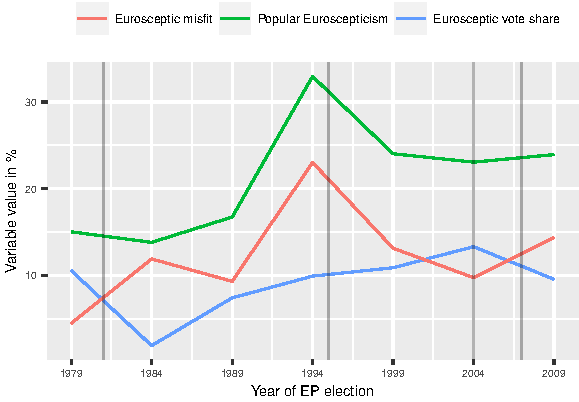
\includegraphics{graphs/graph-1} \end{center}

\end{frame}

\begin{frame}{3.2. Eurosceptic misfit across regions}

\begin{center}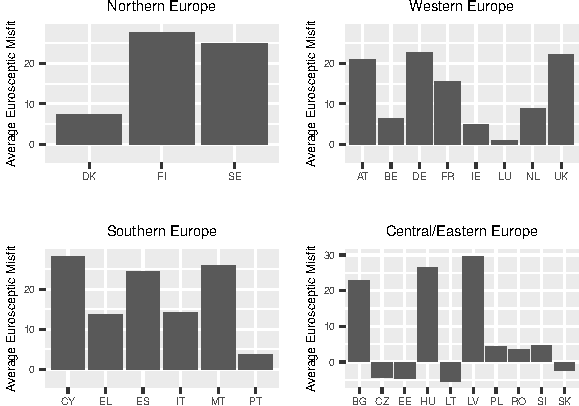
\includegraphics{graphs/displaying_plot-1} \end{center}

\end{frame}

\begin{frame}{3.3. Regression models}

\begin{table}[!htbp] \centering 
  \caption{Regression results} 
  \label{} 
\tiny 
\begin{tabular}{@{\extracolsep{5pt}}lcc} 
\\[-1.8ex]\hline 
\hline \\[-1.8ex] 
 & \multicolumn{2}{c}{\textit{Dependent variable:}} \\ 
\cline{2-3} 
\\[-1.8ex] & \multicolumn{2}{c}{Eurosceptic Misfit} \\ 
 & FE & RE \\ 
\\[-1.8ex] & (1) & (2)\\ 
\hline \\[-1.8ex] 
 General Euroscepticism & 0.48$^{***}$ & 0.45$^{***}$ \\ 
  & (0.10) & (0.09) \\ 
  & & \\ 
 Instrumental Euroscepticism & 0.38$^{***}$ & 0.43$^{***}$ \\ 
  & (0.06) & (0.05) \\ 
  & & \\ 
 Polarisation Index & $-$1.52$^{*}$ & $-$1.92$^{**}$ \\ 
  & (0.84) & (0.74) \\ 
  & & \\ 
 Effective Number of Parties & 0.02 & $-$0.06 \\ 
  & (0.12) & (0.10) \\ 
  & & \\ 
 Membership Duration & 0.08 & 0.04 \\ 
  & (0.08) & (0.06) \\ 
  & & \\ 
 Central/Eastern European &  & $-$5.52$^{*}$ \\ 
  &  & (3.09) \\ 
  & & \\ 
 Constant &  & 0.57 \\ 
  &  & (3.47) \\ 
  & & \\ 
\hline \\[-1.8ex] 
\hline 
\hline \\[-1.8ex] 
\textit{Note:}  & \multicolumn{2}{r}{$^{*}$p$<$0.1; $^{**}$p$<$0.05; $^{***}$p$<$0.01} \\ 
\end{tabular} 
\end{table}

\end{frame}

\begin{frame}{4. Conclusion}

\begin{itemize}
\tightlist
\item
  The Eurosceptic misfit has stayed relatively constant over time,
  except for a spike in 1994
\item
  Eurosceptic misfit considerably smaller in CEE countries
\item
  Eurosceptic vote share generally fails to ``catch up'' with increases
  in popular Eurosceptic attitudes
\item
  Higher degrees of party polarisation shrink the Eurosceptic misfit
\end{itemize}

\end{frame}

\begin{frame}{Thank you for listening!}

Please check out my Github repository for all source codes for the
analysis and presentation documents:

\href{https://github.com/mberneaud/EuroscepticMisfitMasterThesis}{\emph{github.com/mberneaud/EuroscepticMisfitMasterThesis}}

\end{frame}

\begin{frame}{Extra: Model considerations}

\begin{itemize}
\tightlist
\item
  Combination of pooled OLS, fixed effects and random effects models
  used in the thesis

  \begin{itemize}
  \tightlist
  \item
    Fixed effects to cleanly isolate causal effects (read: removing
    unobserved heterogeneity) to measure country-specific variation
  \item
    Random effects to allow for inclusion of time-invariant variables
    (like region) and higher efficiency
  \item
    Pooled OLS for comparison
  \end{itemize}
\end{itemize}

\end{frame}
